\documentclass[10pt]{article}
\usepackage[utf8]{inputenc}
\usepackage[T1]{fontenc}
\usepackage{graphicx}
\usepackage[export]{adjustbox}
\graphicspath{ {./images/} }
\usepackage{amsmath}
\usepackage{amsfonts}
\usepackage{amssymb}
\usepackage[version=4]{mhchem}
\usepackage{stmaryrd}
\usepackage{bbold}

\def\AA{\mathring{\mathrm{A}}}

\begin{document}


\begin{enumerate}
  \setcounter{enumi}{2}
  \item Calculate ratio of spontaneous to stimulated emission for tungsten filament operating at $2000 \mathrm{k}$.
\end{enumerate}

$$
\begin{aligned}
& v=5 \times 10^{14} \mathrm{~Hz} . \\
& \frac{S P \cdot E}{S 7 \cdot E}=e^{h \tau / K E}-10=162443.8 . \\
& k=1.38 \times 10^{-23} \\
& n=6.626 \times 10^{-36} \\
& T=20012 k \\
& 2=500 T 1+2
\end{aligned}
$$

\begin{center}
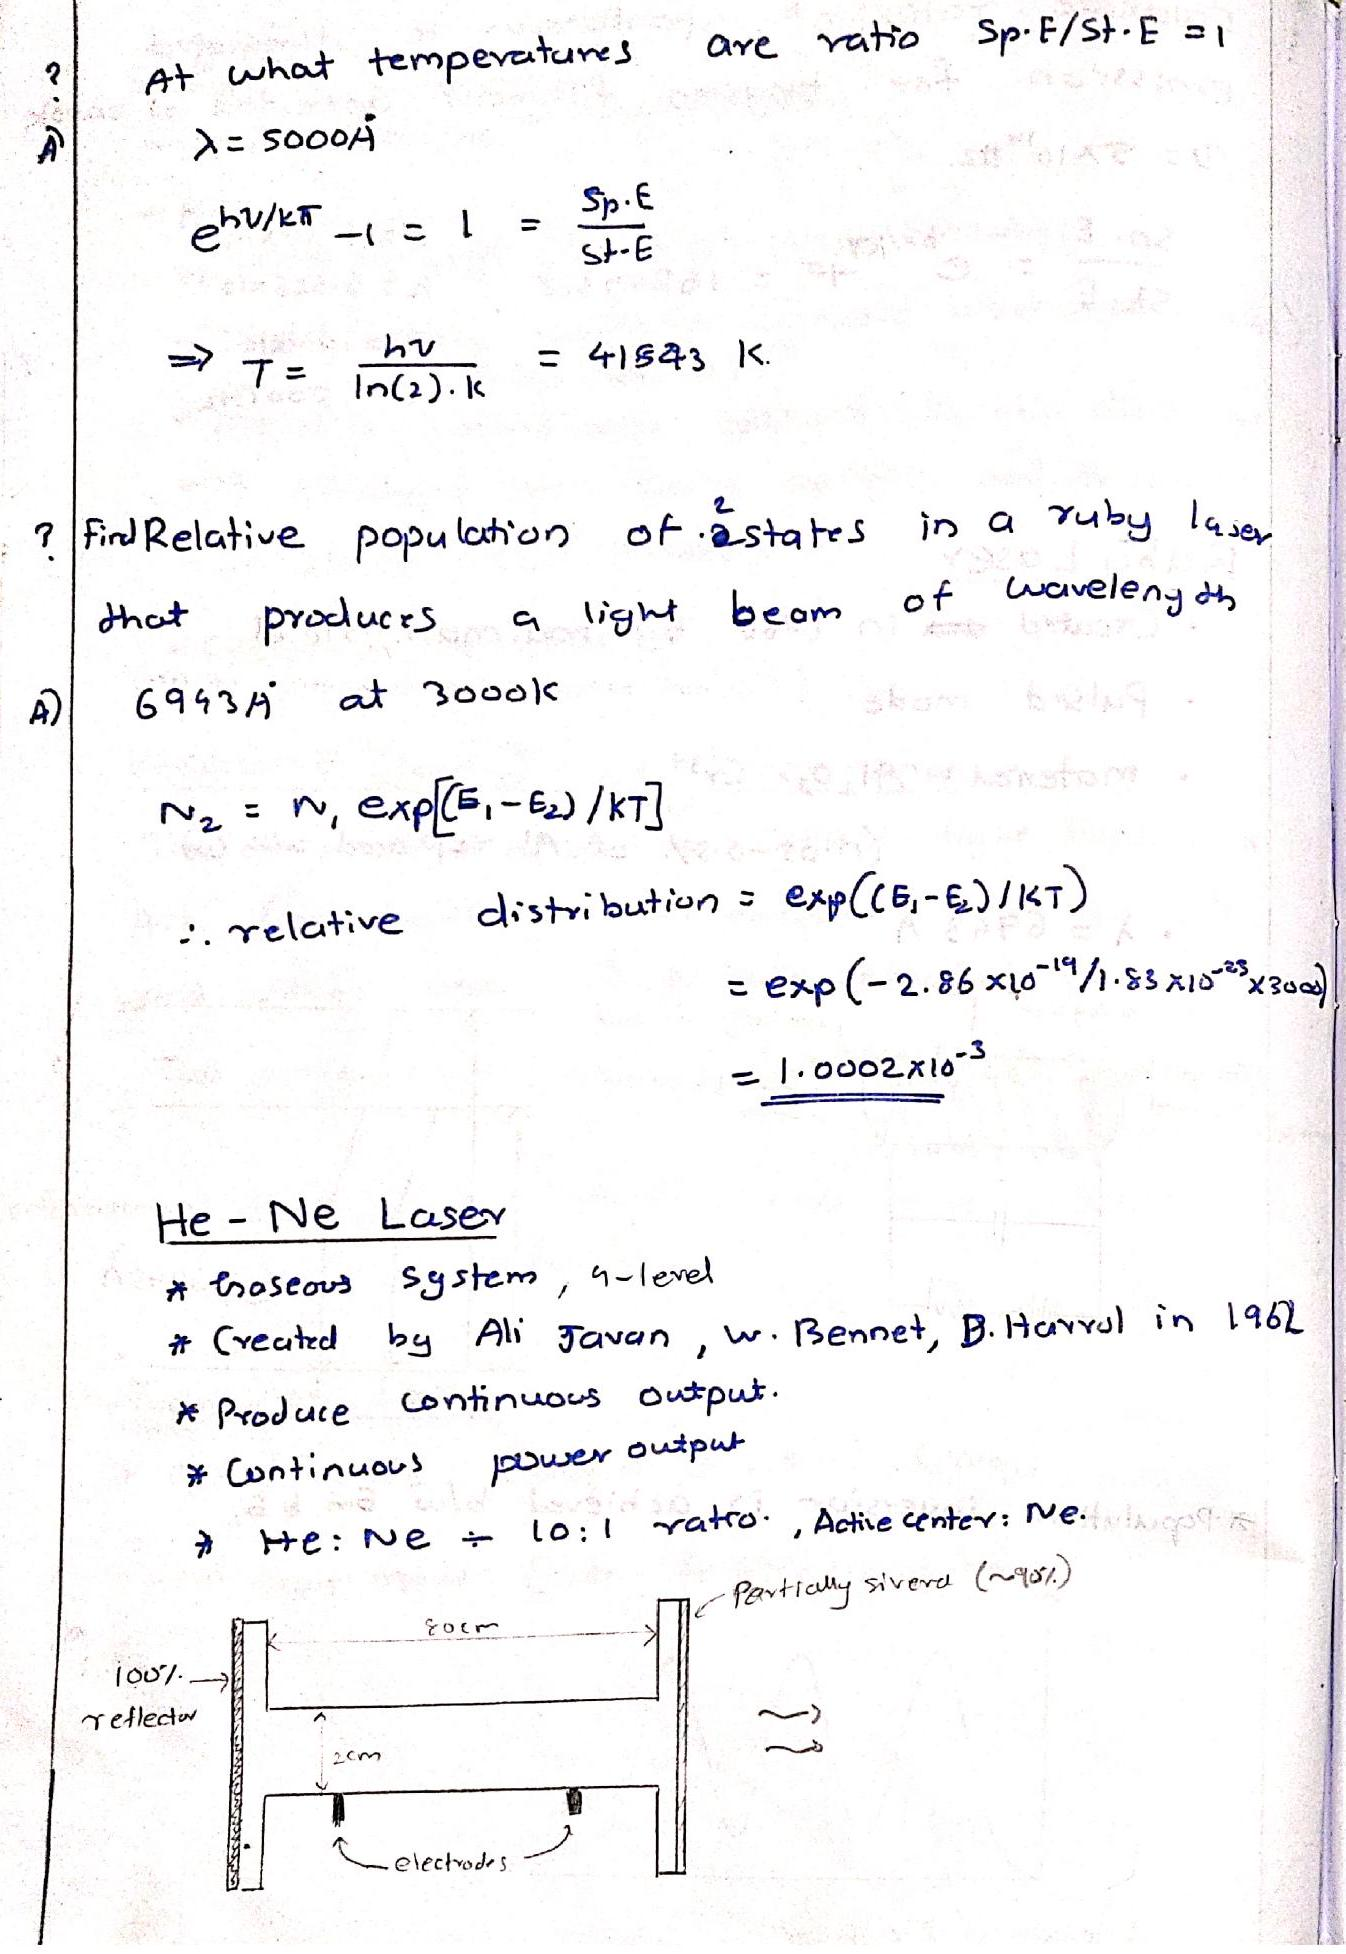
\includegraphics[max width=\textwidth]{2024_06_16_30d750483617f1939202g-04(1)}
\end{center}

Working

Due to electur dischange in gas, energetic electron interacts with ground state helium atomos. The impact of $e^{-}$results in exchonge of some of its energy to the atam. Hs a result. Helum atums gets excited to higher enoryy levels. $F_{1} d F_{2}$. These two energy levals are cluse to $E_{4} \& E_{6}$ levels of Ne atoms. and collision of second liind takes place blui them, hence we goes to excited state. Es of $E_{3}$. E levels of we forms metastable state.

3 trpes of tronsition are possible :

\begin{itemize}
  \item $E_{4} \rightarrow E_{3}$, emitting $\mathbb{R}$ of $\lambda=1.15 \mu \mathrm{m}$
  \item E6 $\rightarrow E 5$, emitting $F R$ of $\lambda=3.39 \mu m$
  \item E6 E3, emitting red light of $\lambda=632-8 \mathrm{~nm}$
\end{itemize}

Neon atoms in terminal level $E_{3}$ decay very rapialy to $E_{2}$ metastable state, much faster than spontaneous rotelecay frum $E_{6} \rightarrow E_{3}$ level. Thus lower level ${ }^{5}$ is keupt empty and population inversion is achieved b/w $E_{6} \& E_{3}$

\begin{center}
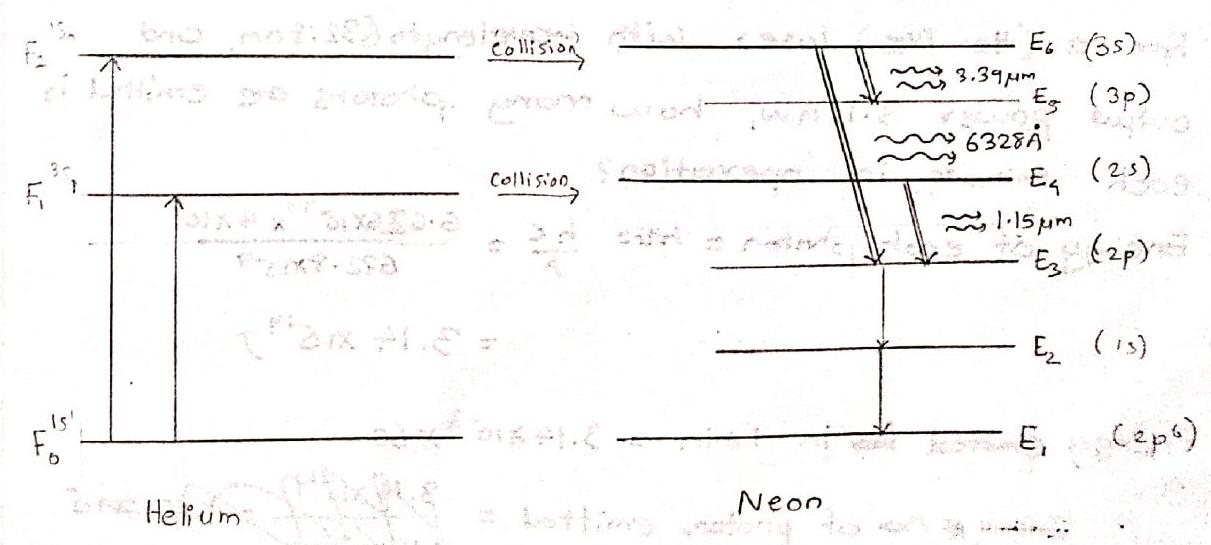
\includegraphics[max width=\textwidth]{2024_06_16_30d750483617f1939202g-04}
\end{center}

\section*{Fibrer Optics}
\section*{Total internal reflection}
By snellis law:

$$
n_{1} \sin \left(\theta_{1}\right)=n_{2} \sin \left(\theta_{2}\right)
$$

At critical angle., $\theta_{2}=90$

$$
\therefore n_{1} \sin \left(\theta_{c}\right)=n_{2}
$$

$$
\theta_{c}=\sin ^{-1}\left(\frac{n_{2}}{n_{1}}\right)
$$

\begin{center}
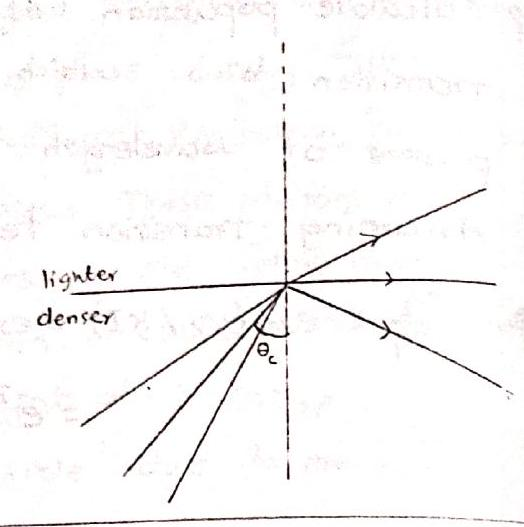
\includegraphics[max width=\textwidth]{2024_06_16_30d750483617f1939202g-05(3)}
\end{center}

\begin{itemize}
  \item Water - $\theta_{i v}{ }^{\circ} \theta_{2}=49^{\circ}$
  \item Dicmond-air, $\theta_{c}=24_{\tau}$.
  \item Gluss - air, $\theta_{c}=42$
\end{itemize}

\begin{center}
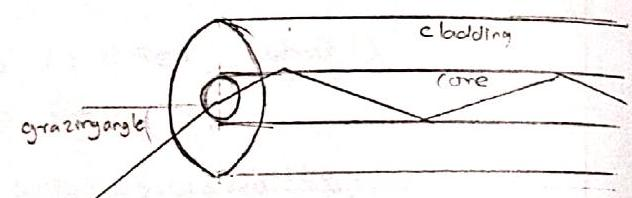
\includegraphics[max width=\textwidth]{2024_06_16_30d750483617f1939202g-05}
\end{center}

Structuve of Fibrer Optic Cable

\begin{center}
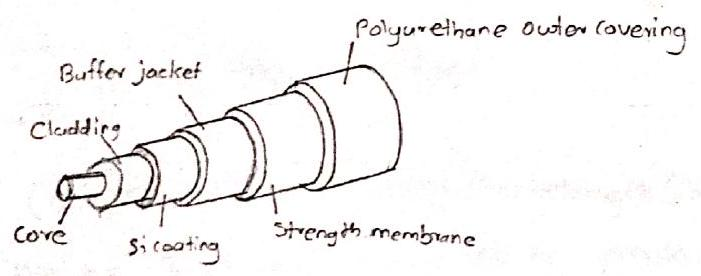
\includegraphics[max width=\textwidth]{2024_06_16_30d750483617f1939202g-05(2)}
\end{center}

\begin{itemize}
  \item Polyurethane: for mecharical crushing
  \item Butfor jacket : to prevent moistume
  \item Si-coarting : protect from dust \& soratches
\end{itemize}

\section*{Classification}
\begin{itemize}
  \item wrt. Index profile: step-index, graded index

  \item wrt. made : single mode, multimude.

\end{itemize}

step index single mode

\begin{center}
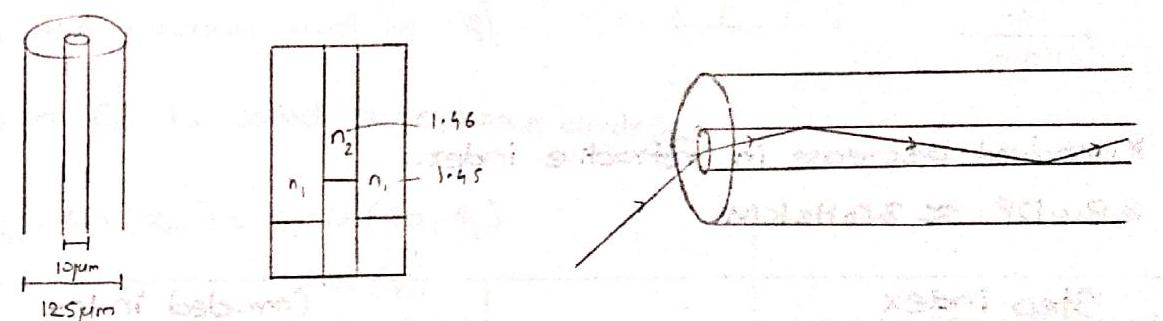
\includegraphics[max width=\textwidth]{2024_06_16_30d750483617f1939202g-05(1)}
\end{center}

\begin{itemize}
  \item Allows only one path for light
  \item Bandwidth distance product: $>3 \mathrm{CrH}_{2} \cdot \mathrm{km}$
  \item Splicing is difficut.
\end{itemize}

Step index multimode.\\
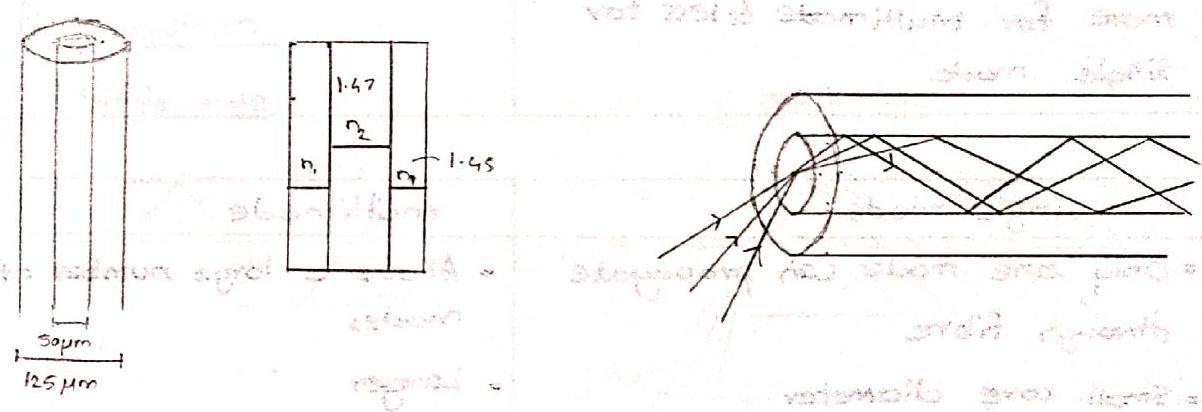
\includegraphics[max width=\textwidth, center]{2024_06_16_30d750483617f1939202g-05(4)}

\begin{itemize}
  \item Allows multiple path for light
  \item easior to splice
  \item BwDP $\sim 300 \mathrm{MH}_{2}$. Km
\end{itemize}

Crraded index multimode

\begin{center}
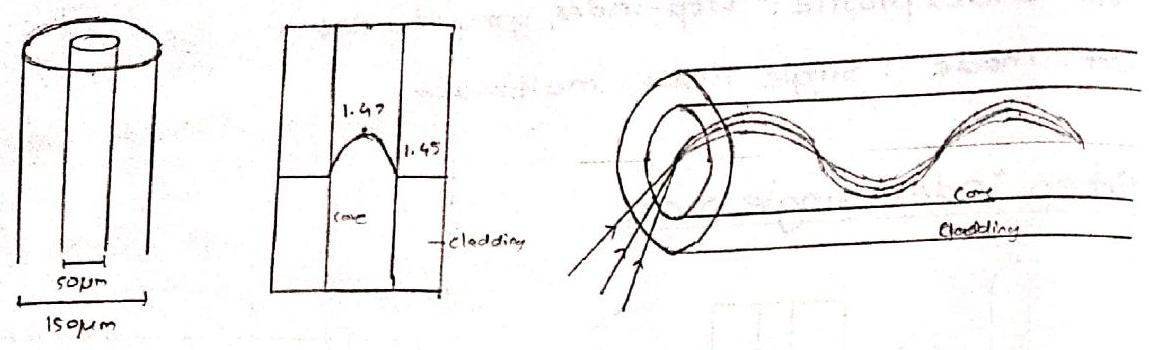
\includegraphics[max width=\textwidth]{2024_06_16_30d750483617f1939202g-06(3)}
\end{center}

\begin{itemize}
  \item Gradual decrease in refractive index.
\end{itemize}

*BUDP $\approx 3 \mathrm{CNH}_{2} \mathrm{KM}$

\begin{center}
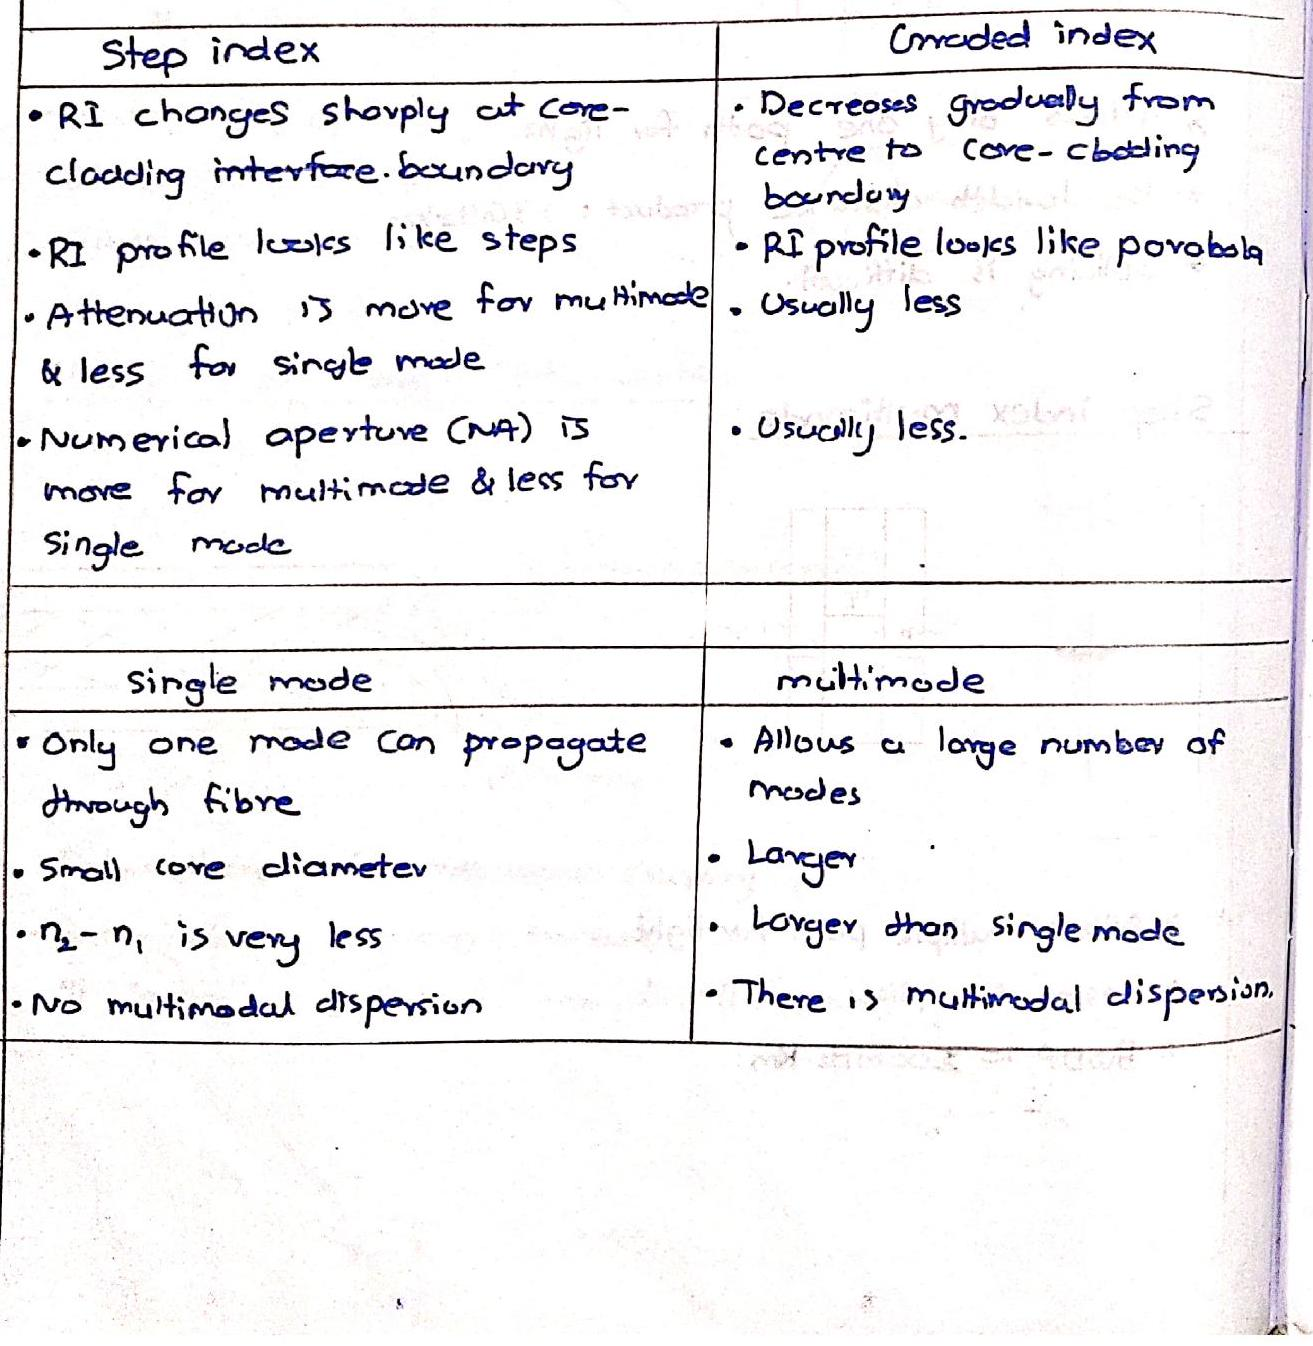
\includegraphics[max width=\textwidth]{2024_06_16_30d750483617f1939202g-06(4)}
\end{center}

Numerical Aperture (NA)

$\sim \sin$ of largest angle af incident rag.can have fon tir in core. By snell's law:

Es

na. $\sin (\alpha)=n, \sin (\alpha)$

For TIR, angle of ircidence

in the medium must be $>\theta_{\varepsilon}$.

$\alpha$ at $\theta_{c}$ is called acceptance angle. $\left(\alpha_{m}\right)$

$n_{a} \cdot \sin \left(\alpha_{m}\right)=n, \sin \left(90-\theta_{c}\right)$

$$
\begin{aligned}
& =n_{1} \cos (\theta) \\
& \equiv n_{1} \sqrt{1-\sin ^{2}(\theta)} \\
& =n_{1} \sqrt{1-n_{2}^{2} / n_{1}^{2}}
\end{aligned}
$$

$n_{a} \cdot \sin \left(\alpha_{m}\right)=\sqrt{n_{1}^{2}-n_{2}^{2}}$

NA.

\begin{center}
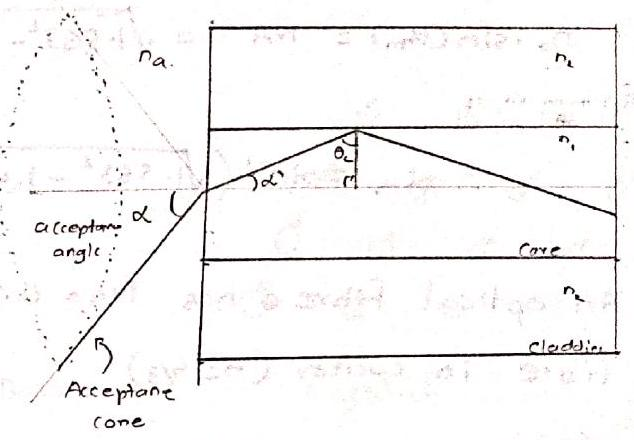
\includegraphics[max width=\textwidth]{2024_06_16_30d750483617f1939202g-06(1)}
\end{center}

\section*{Propagation}
\section*{Single mode}
\begin{center}
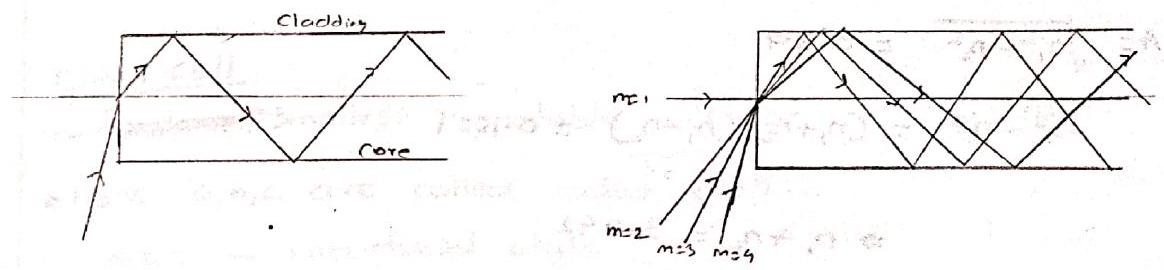
\includegraphics[max width=\textwidth]{2024_06_16_30d750483617f1939202g-06(2)}
\end{center}

Graded index

\begin{center}
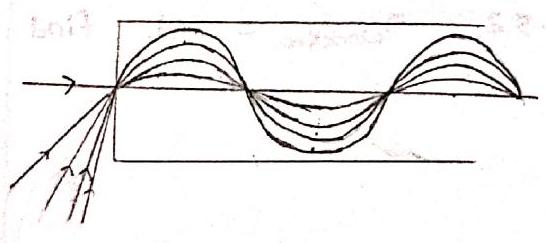
\includegraphics[max width=\textwidth]{2024_06_16_30d750483617f1939202g-06}
\end{center}

\begin{itemize}
  \item Eventhough all waves emehove different velocity, they reach at satine time, due to precise differences in distance which they travel.
\end{itemize}

ie, they

\section*{Simple cubic}
\begin{itemize}
  \item Atoms only at corners.
\end{itemize}

Coordination no. (cw) $(:=$ of equidistant neightours)

$=6$

\begin{itemize}
  \item No. of citoms $=8 \times 1 / 8=1$
\end{itemize}

\begin{center}
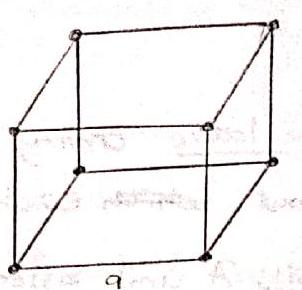
\includegraphics[max width=\textwidth]{2024_06_16_30d750483617f1939202g-07}
\end{center}

\begin{itemize}
  \item $r=a / 2$
\end{itemize}

-PE $=\pi / 6 \approx 52.36 \%$

Body Centered Cubic.

\begin{center}
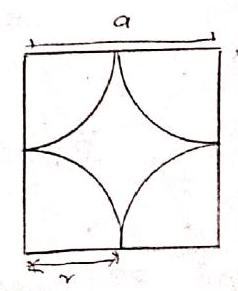
\includegraphics[max width=\textwidth]{2024_06_16_30d750483617f1939202g-07(2)}
\end{center}

\begin{itemize}
  \item Atome cit corners \&
\end{itemize}

budy centers.

\begin{itemize}
  \item Cn $=8$ (cort. body diagorad)
\end{itemize}

\#ofatoms $=1 / 8 \times 8+1=2$

\begin{itemize}
  \item $r=\frac{\sqrt{(\sqrt{2} a)^{2}+a^{2}}}{4}=\frac{\sqrt{3}}{4} a$
\end{itemize}

\begin{center}
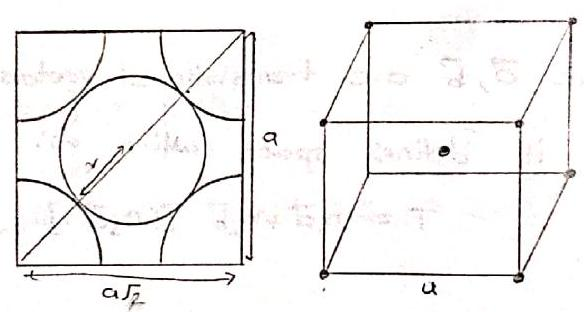
\includegraphics[max width=\textwidth]{2024_06_16_30d750483617f1939202g-07(3)}
\end{center}

\begin{itemize}
  \item $P E=\pi \cdot \sqrt{3} / 8=68.02 \%$
\end{itemize}

Face centered Cubic.

Atoms at corners $\AA$

face centers

\begin{itemize}
  \item $C N=12$
\end{itemize}

\# of atoms $=8 \times \frac{1}{8}+6 \times \frac{1}{2}$

$$
=\underline{\underline{4}}
$$

\begin{center}
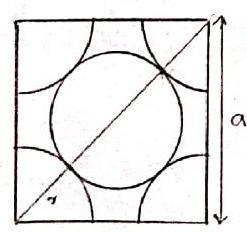
\includegraphics[max width=\textwidth]{2024_06_16_30d750483617f1939202g-07(1)}
\end{center}

\begin{itemize}
  \item $r=\frac{\sqrt{a^{2}+a^{2}}}{4}=\frac{\sqrt{2}}{4} a$.
\end{itemize}

$P E=\pi \sqrt{2} / 6=74.05 \%$\\
Packing efficiency/factor/density

\begin{center}
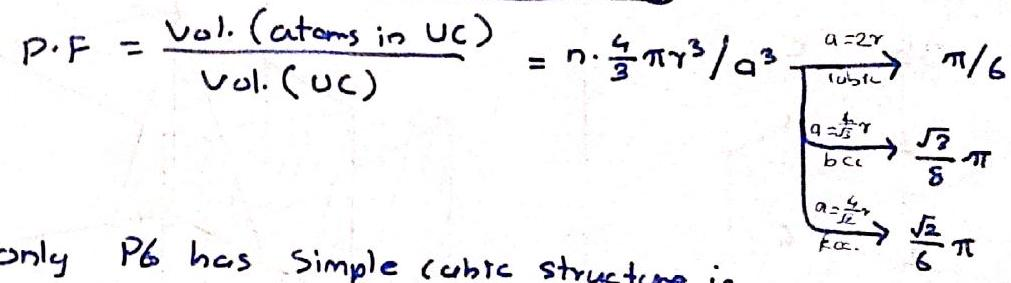
\includegraphics[max width=\textwidth]{2024_06_16_30d750483617f1939202g-07(4)}
\end{center}

elemential state.

\section*{Packing density}
$$
\rho=\frac{n \cdot A}{N_{A} \cdot a^{3}} \quad \begin{aligned}
& A \text {-atamic mass } / \text { mas of } \\
& n=\Delta \# \text { of atmon/unit ce } \|
\end{aligned}
$$

$$
N_{A}=6.022 \times 10^{23}
$$

Lattice plane s(\&miler indices)

\section*{miller indices ( $h$ k )}
These are s smallest possible integers which have same ratios as realpromal

of the intercepis of plones. conconnal

on 3 axes.

\section*{Deter minig. miller indices}
\begin{itemize}
  \item Determire intercepts $(x, y, z)$ in temss of lattice constants $(a, b, c)$.
  \item Talse reciprocal of Different unans to draw
  \item Reduce to whole numbers by lattice planos. multiplying by LCM of deno minators.
\end{itemize}

\begin{center}
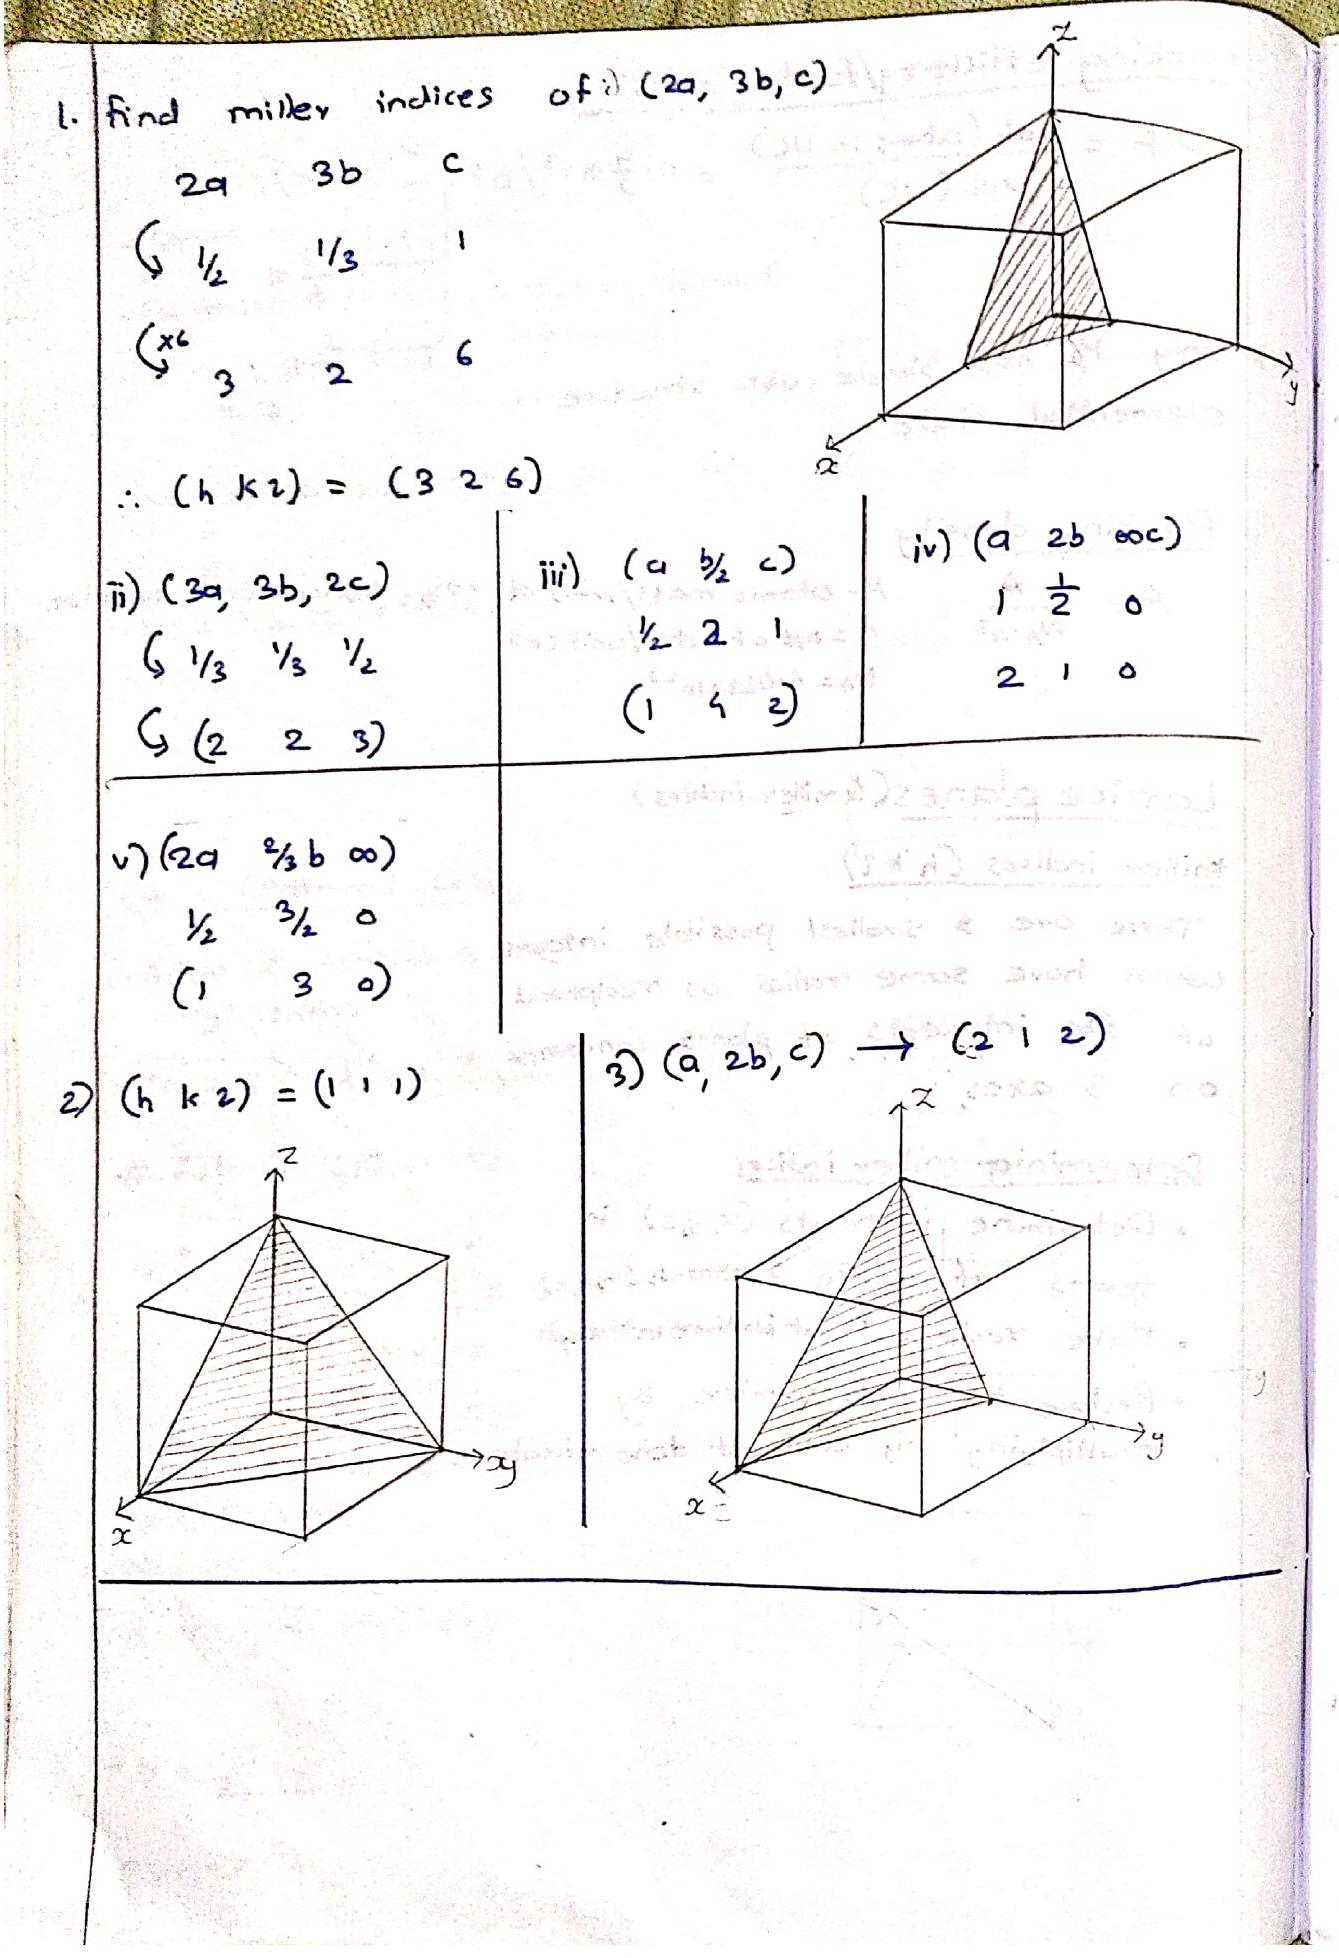
\includegraphics[max width=\textwidth]{2024_06_16_30d750483617f1939202g-08(1)}
\end{center}

\begin{center}
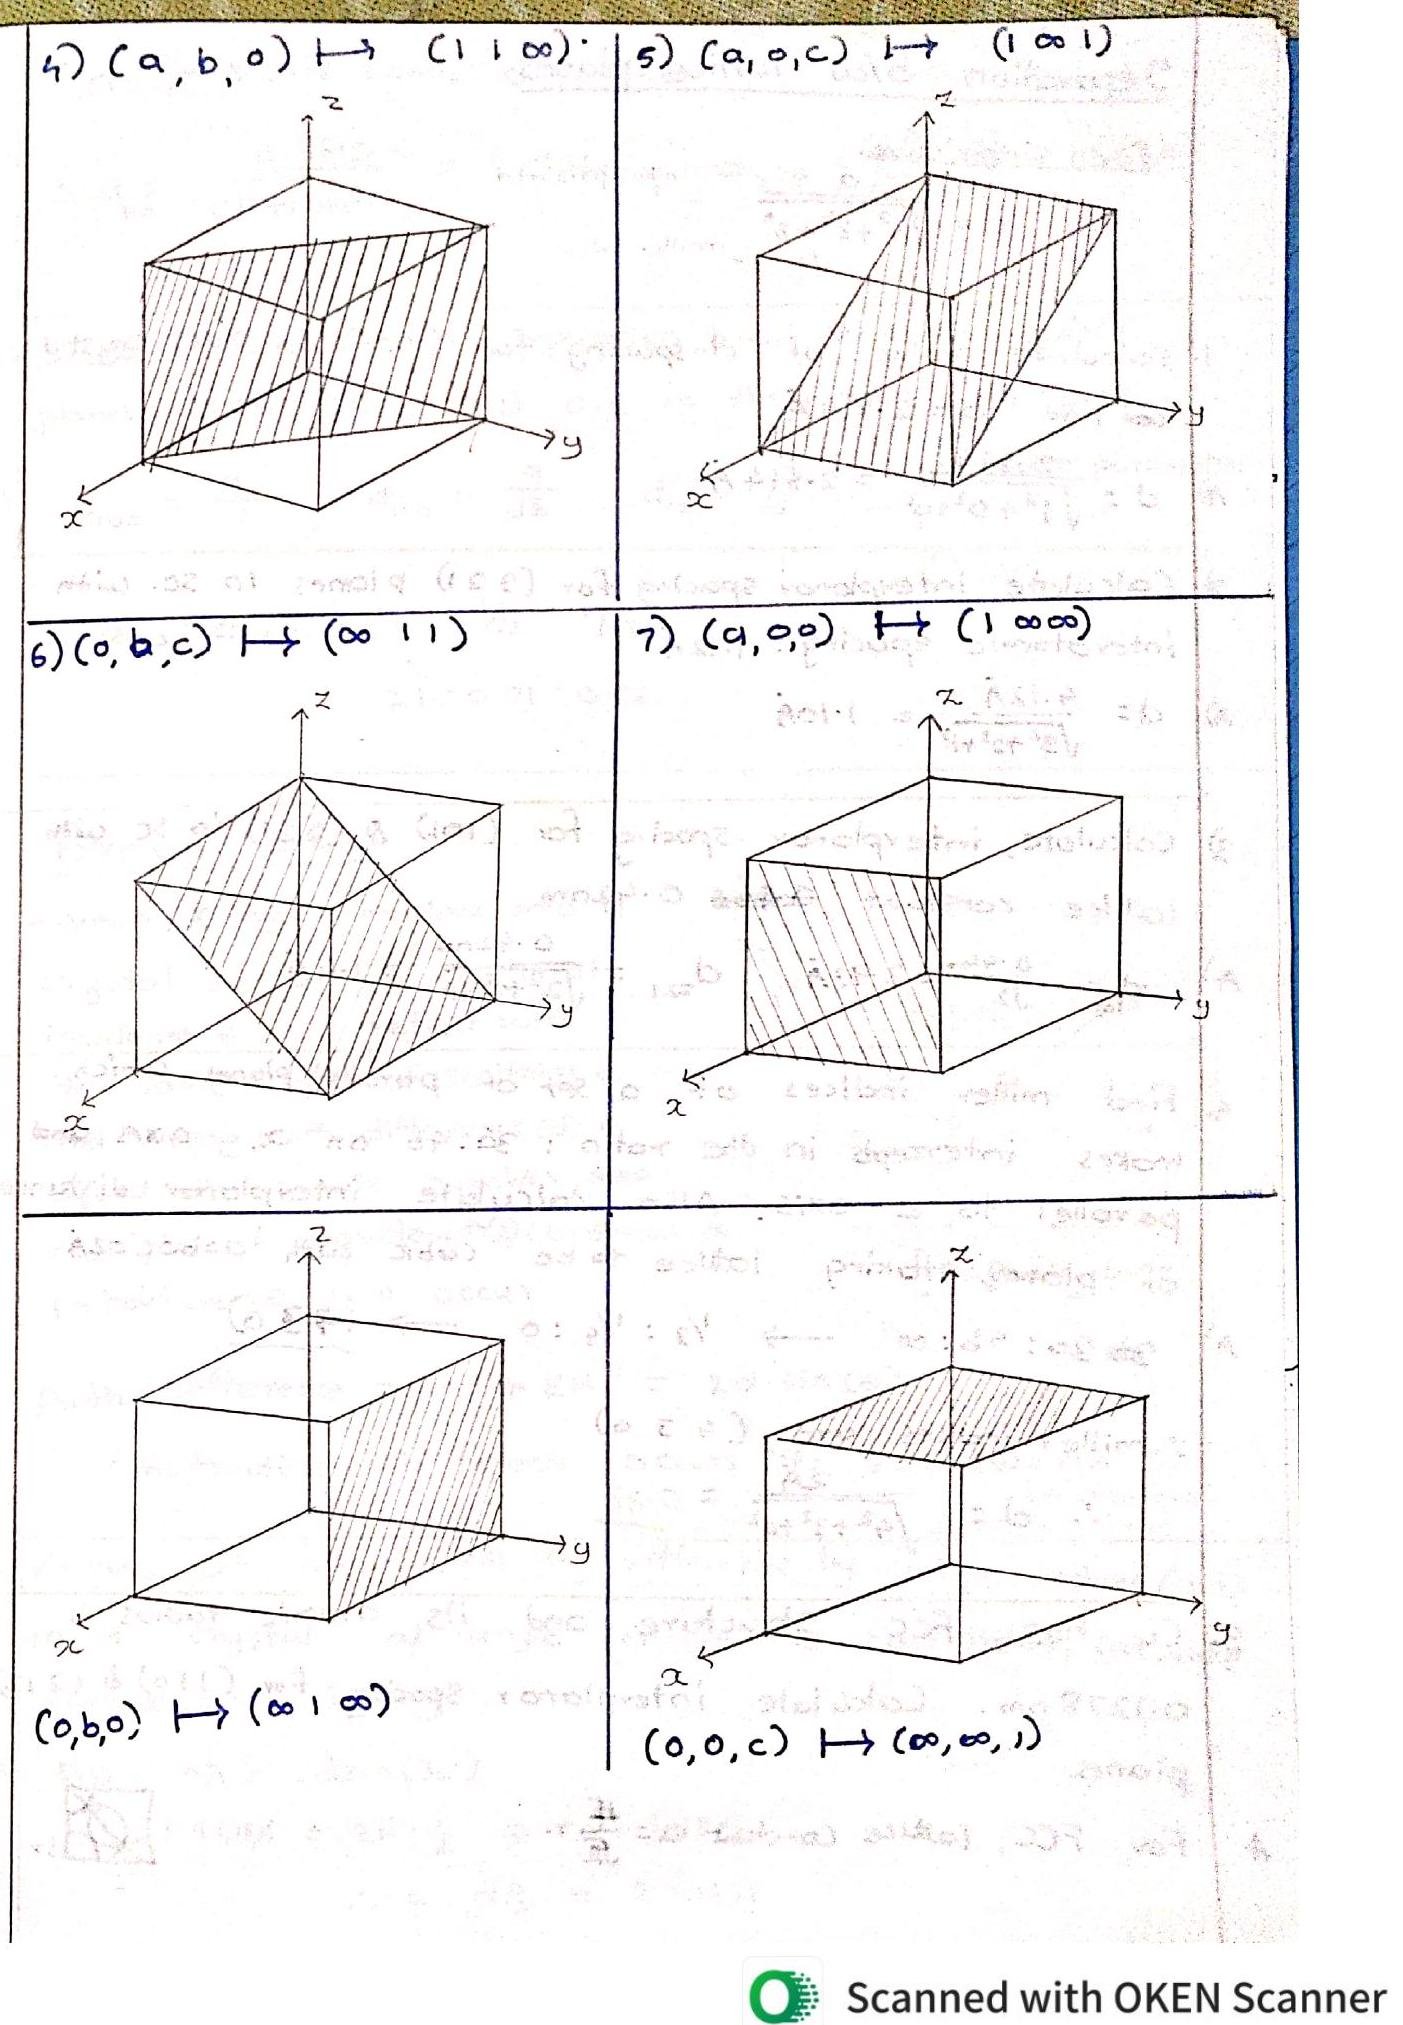
\includegraphics[max width=\textwidth]{2024_06_16_30d750483617f1939202g-08}
\end{center}

Separation b/w lattice planes

for simple calls:

$$
d=\frac{a}{\sqrt{h^{2}+k^{2}+z^{2}}} \text { simple caller indices }
$$

\begin{enumerate}
  \item Calculate value of cl-spacing for (100) in rracl orystud li for $a=2.814 \dot{A}$\\
A) $d=\frac{2.814}{\sqrt{1^{2}+0^{2}+0^{2}}}=2.814 \dot{A}$
\end{enumerate}

\begin{enumerate}
  \setcounter{enumi}{1}
  \item Calculate interplonor spacing for (321) plomes in sc. with interatomic spacing: $9.12 A^{\circ}$\\
A) $d=\frac{4.12 \dot{A}}{\sqrt{3^{2}+2^{2}+1^{2}}}=1.10 \dot{A}$

  \item Calculate, interplanor sparing for (101) \& (221) in SC with lattice constant $0.42 \mathrm{~nm}$\\
A) $\quad d_{101}=\frac{0.42 \pi n}{\sqrt{2}}=2.97 \dot{A}, \quad d_{221}=\frac{0.42 n \pi 0}{\sqrt{2^{2}+2^{2}+1^{2}}}=1.4 \dot{A}$

\end{enumerate}

\begin{enumerate}
  \setcounter{enumi}{3}
  \item Find miller indices of a set of parallel planes which mokes intercepts in the ratio: $3 a: 4 b$ on $x, y$ axes and parallel to $z$-axis. Also calculate interplonar distance of plones, taking lallice to be cubs with $a=b=c=2 \dot{A}$\\
A) $3 a: 4 b: \infty \longrightarrow 1 / 3: 1 / 4: 0 \rightarrow(430)$
\end{enumerate}

$\therefore$ miller indices are $\left(\begin{array}{lll}4 & 3 & 0\end{array}\right)$

$$
\therefore d=\frac{2 \dot{S}}{\sqrt{4^{2}+3^{2}+0^{2}}}=0.4 \dot{A}
$$

\begin{enumerate}
  \setcounter{enumi}{4}
  \item Cu has FCC structure and its atomic radius is $0.1278 \mathrm{~nm}$. Calculate interplarar spacing for (110) \& (212) planes.
\end{enumerate}

A For FCC, lattice constant $a=\frac{4}{\sqrt{2}} r$.

$$
\begin{aligned}
& a=\frac{4}{\sqrt{2}} \times 0.1218 \mathrm{~nm}=0.3615 \mathrm{~nm} \\
& \therefore d_{110}=\frac{0.3615 \mathrm{~nm}}{\sqrt{1^{2}+1^{2}+0^{2}}}=2.556 A^{\circ}, \quad d_{2,2}=\frac{0.3615}{\sqrt{2^{2}+1^{2}+2^{2}}}=1.205 A^{-}
\end{aligned}
$$

\begin{enumerate}
  \setcounter{enumi}{5}
  \item Show that in a SC. Separation b/w success iv lattice .planes, (100), (110), (111) are in the ration: 1:0.71:0.58
\end{enumerate}

A) $\quad d_{100}=\frac{9}{1}, \quad d_{110}=\frac{9}{\sqrt{2}}, \quad d_{11}=\frac{9}{\sqrt{3}}, \quad a=$ lattice parameter,

$$
\begin{aligned}
\therefore d_{100}: d_{110}: d_{111} & =1: 1 / \sqrt{2}: 1 / \sqrt{3} \\
& =1: 0.71: 0.58
\end{aligned}
$$

Bragg's Law

$\sim$ when $x$-vol is incident onto a crystal surface angle of incidence, $\theta$. "will reflect with the same angle of scattering. $\theta$. And when pats difference (d) is equal to whole number, multiple of woveleng $\partial(\lambda)$ (constructive interference will occur.

\begin{center}
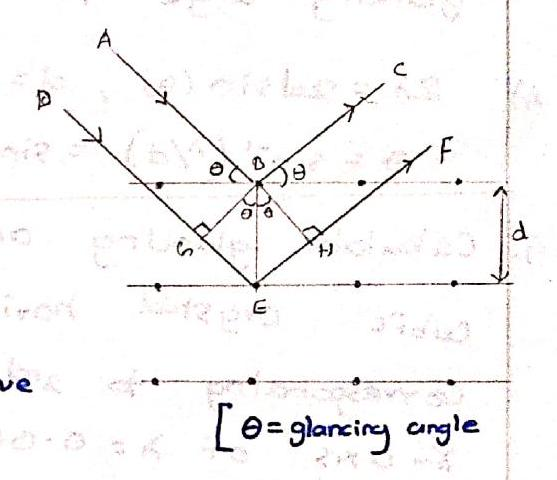
\includegraphics[max width=\textwidth]{2024_06_16_30d750483617f1939202g-09}
\end{center}

Doth difference $=G E+E H=2 d \cdot \sin (\theta)$

constructive interference occurs of: $\quad 2 d \sin (\theta)=n_{\text {diffraction }}^{n \lambda}$ diffraction order

\begin{enumerate}
  \item $x$-rays of $\lambda=1.5918 A$ are diffracted by miller indices (111) in a crystal at angle $30^{\circ}$. in the first order, calculate interatomic spacing.
\end{enumerate}

A) $P \cdot D=n \lambda=2 d \sin \left(30^{\circ}\right)$

$$
\begin{aligned}
& 1.5415 \dot{A}=2 d \cdot \frac{1}{2} \Rightarrow d=1.5418 \dot{A} \\
& \therefore a=d \sqrt{3}=2.7044
\end{aligned}
$$

\end{document}